\section{Implementation and Artifact Traceability}
The accompanying \code{evidence/claim-evidence-matrix.md} maps empirical claims to exact source artifacts, row filters, and derivations. \code{evidence/source-manifest.json} records original absolute paths, campaign-relative paths, uncompressed SHA-256 hashes, and committed snapshot hashes. Large JSON files are losslessly gzip-compressed. Compressed snapshots can be verified and read without the original checkout. The manuscript asset script recomputes aggregate RMSE from C's saved predictions and verifies exact pair membership, loop retention, and physical coverage from serialized masks.

The campaign sessions are A: 358697902; B: 358708561; C: 358713276; D: 358778452. They are completed private Kaggle executions. Source commit \code{c825bf57652005c80faff79cf4dfd58e3a9baa14} governs the evaluated pipeline. The recovered policy's training source is \code{aeb5dad65d681728d525fb78a4ab919b0432ab90}; its relevant pair-training, policy, and reward modules agree with the campaign base. The new manuscript does not rerun training or replace any campaign artifact.

The input CSV SHA-256 begins \code{6c148f2cae68abac}, and the frozen checkpoint file begins \code{42764f0db204863b}. The frozen parameter-state hash begins \code{56907374794d9203}; the file hash and state hash describe different objects. The recovered selected policy file hash begins \code{b1f41771c102bec6}. Full hashes and identities are retained in the evidence files. None of these hashes certifies the historical scientific semantics of the file contents.

\begin{table}[H]
\centering\small
\caption{Code paths defining the reported method at the campaign base. Function names identify the implementation, not a claim that every alternate repository path was executed.}
\label{tab:code}
\begin{tabular}{>{\raggedright\arraybackslash}p{0.26\textwidth}>{\raggedright\arraybackslash}p{0.38\textwidth}>{\raggedright\arraybackslash}p{0.27\textwidth}}
\toprule
Component & File and entry point & Role \\
\midrule
Node/target conversion & \code{data/loaders/base\_loader.py}: \code{SubhaloData.get\_node\_features}, \code{HaloData.log\_halo\_mass} & Four logs and stored target \\
Graph geometry & \code{graph/graph\_builder.py}: \code{\_build\_standard\_graph}, \code{\_compute\_edge\_features} & Radius graph, loops, fallback, attributes \\
Predictor & \code{model/model.py}: \code{CosmicNetGNN}, \code{NNConvBlock} & Frozen edge-conditioned GNN \\
Pair training & \code{rls/pair\_training.py}: \code{train\_pair\_policy}; \code{rls/pair\_policy.py}: \code{pair\_mask} & Ordered actions, repair, rollout baseline \\
Physical reward & \code{rls/train\_policy.py}: \code{\_graph\_physics\_terms}; \code{rls/rewards.py} & Loop-free reference-relative proxy \\
Exact feasibility & \code{rls/constraints.py}: \code{minimum\_additions}; \code{rls/constrained\_policy.py}: \code{select\_pairs} & Matching-based completion and ranking \\
Scorers and benchmark & \code{rls/benchmark\_scorers.py}; \code{rls/matched\_benchmark.py} & Common budgets and cost accounting \\
Adaptation & \code{rls/pair\_tta.py}: \code{adapt\_pair\_policy} & Label-free rollouts and exact final mask \\
\bottomrule
\end{tabular}
\end{table}

\section{Recorded Settings and Recovery Limits}
\begin{table}[H]
\centering\small
\caption{Recorded campaign and policy settings. Backbone settings specify the loaded architecture; they are not a certified historical backbone training recipe.}
\begin{tabular}{llll}
\toprule
Setting & Value & Setting & Value \\
\midrule
Node / edge dimensions & 4 / 5 & GNN layers / width / output & 3 / 64 / 64 \\
Pooling / dropout & mean / 0.05 & Radius / self-loops & 2.0 Mpc / retained \\
Policy width / normalization & 64 / train-fitted & Epochs / selected epoch & 60 / 42 (zero-based) \\
Policy Adam rate / batch & $10^{-3}$ / 32 graphs & Rollouts / gradient clip & 4 / 1.0 \\
Keep curriculum & 0.9 to 0.4 in 40 epochs & Entropy / value weights & 0.01 / 0.5 \\
Reward error scale (recovered) & 0.124135822 dex & Constraint / decoder & no isolates / direct \\
TTA Adam rate / MC draws & $10^{-4}$ / 15 & TTA patience / keep & 3 / 0.5 \\
TTA KL / rate decay & 0 / 1 & Random validation seeds & 10 \\
\bottomrule
\end{tabular}
\end{table}

The recovered training metadata explicitly marks the reward scale as reconstructed from the exact training inputs and frozen predictions. Its CPU float32 reconstruction is not asserted to be bitwise identical to the original GPU scalar. Normalization buffers are compatible with the recovered data and the replayed validation RMSE differs by approximately $6\times10^{-8}$ dex. Original policy weights and logs are retained. Missing optimizer and RNG states mean recovery supports inference evaluation, not exact resumption of an interrupted optimizer trajectory.

One optional Stage B training graph, \code{tng100\_0000005}, has $P=12$ pairs, requested $\lceil0.4P\rceil=5$, but minimum no-isolate edge cover 6. The exact decoder correctly rejects that request. A topology-only eligibility report excludes it from optional backbone fine-tuning; all 81 validation and 82 test graphs remain eligible. Exclusion was not based on its residual, and no budget was increased. This case illustrates why a minimum-fraction threshold is insufficient to guarantee feasibility.

\section{Per-Halo Diagnostics}
\begin{figure}[H]
\centering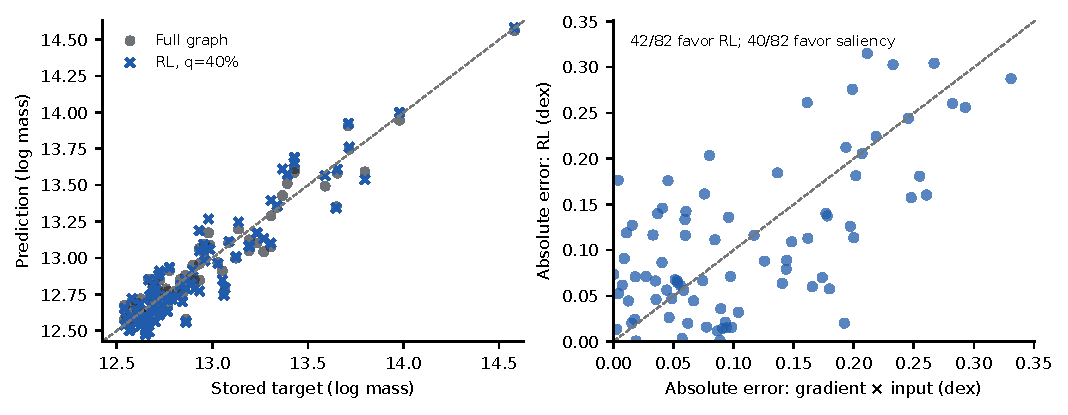
\includegraphics[width=0.96\textwidth]{figures/per_halo_diagnostics.pdf}
\caption{C's saved per-halo predictions at requested 40\% retention. Left: full and RL predictions versus the stored logarithmic target. Right: RL and gradient~$\times$~input absolute errors on identical halos; points below the diagonal favor RL. These plots expose heterogeneity within the aggregate near-tie, without adding independent experimental units.}
\label{fig:halos}
\end{figure}
Figure~\ref{fig:halos} uses the same 82 halos as the main tables. Multiple methods and budgets do not enlarge this sample. The paired statistical export also records leave-one-halo-out RMSE contrasts and Holm-adjusted results for all 21 nontrivial-budget contrasts. These diagnostics support sensitivity assessment, not independent confirmation after test-set inspection.

\section{Missing Evidence and Proposed Confirmation}
No fabricated result panels are supplied for unavailable experiments. The following gaps are explicit placeholders for future evidence: certified catalog field/target semantics and original checkpoint training provenance; independent policy/backbone seeds and volumes; actual cross-simulation and observational validation; physical-reward, feature, and constraint ablations; per-halo final TTA predictions and masks; calibrated uncertainty and repeated hardware/memory measurements. The machine-readable campaign exports do not provide those results. The companion \code{evidence/missing-results.md} prioritizes them and specifies what would resolve each gap.

The current evidence can support supervisor discussion of feasibility, methodology, effect sizes, and computational failure modes. It is insufficient to declare a new astrophysical mass calibration, robust RL superiority, or deployment efficiency. A later confirmatory study must use new independent evidence and report changes to dataset, objective, checkpoint, and selection protocol explicitly.
